Here we study the effect of hidden dimension size on each dataset. We experiment with $h \in \{16, 32, 64, 128\}$ while keeping other hyperpameters the same.

\begin{figure}[ht]
  \centering
  
  \begin{subfigure}[ht]{\linewidth}
    \centering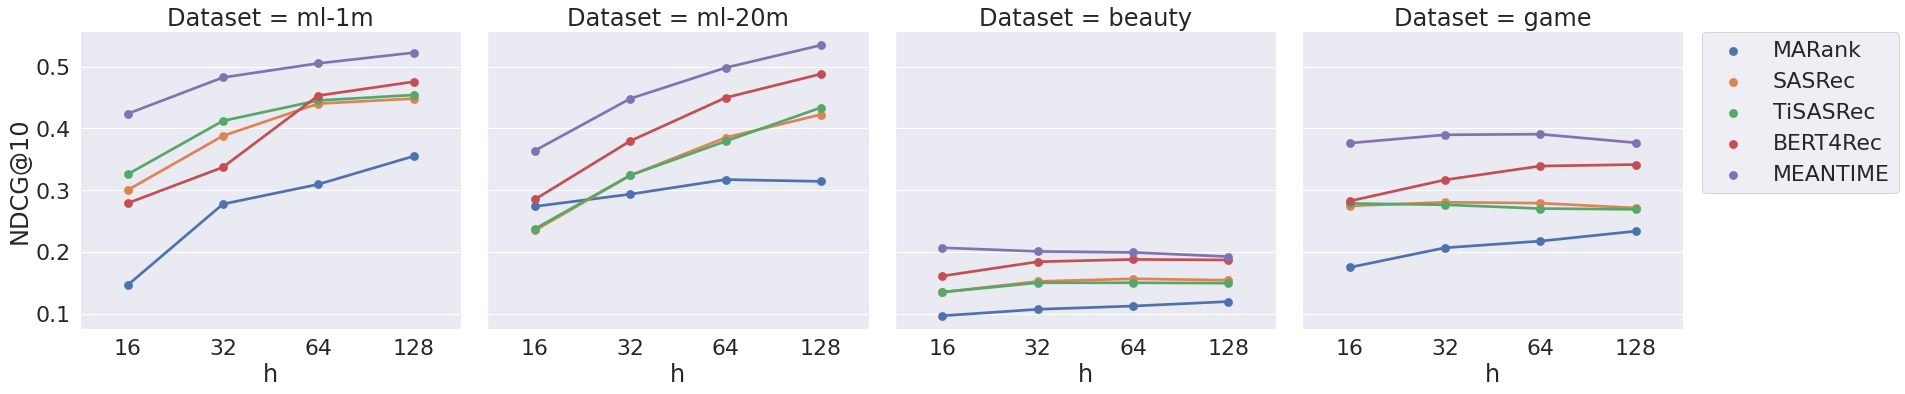
\includegraphics[width=\linewidth]{figures/impact_h/n10.png}
    \caption{NDCG@10}
  \end{subfigure}
  \begin{subfigure}[ht]{\linewidth}
    \centering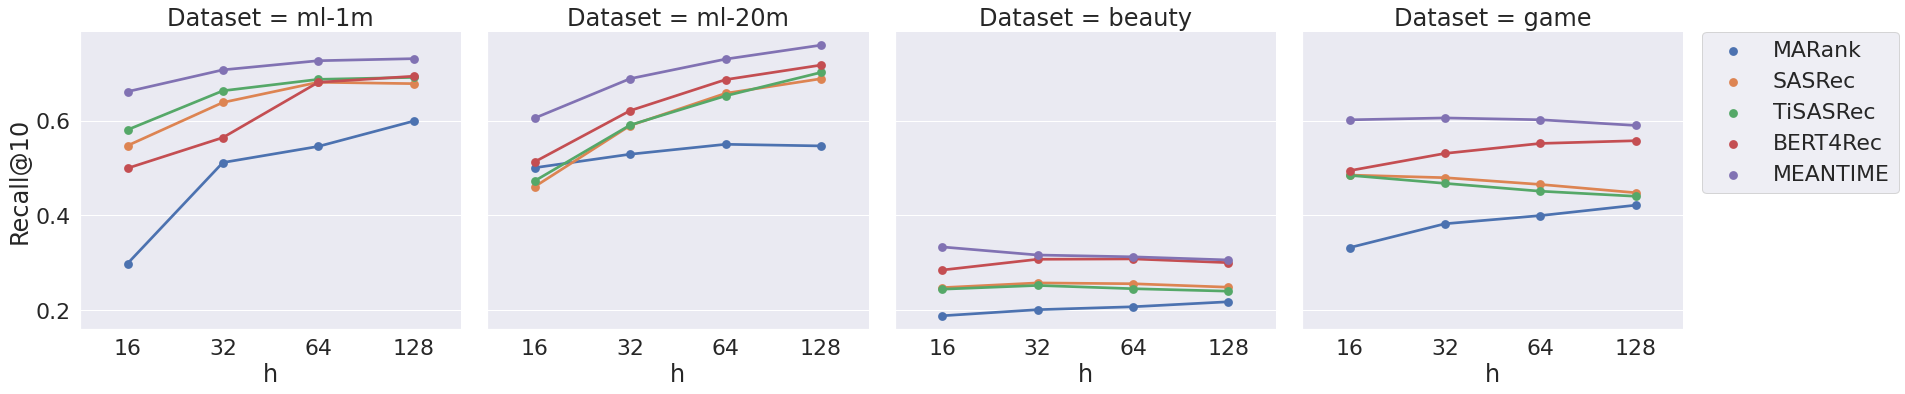
\includegraphics[width=\linewidth]{figures/impact_h/r10.png}
    \caption{Recall@10}
  \end{subfigure}
  
  \caption{Effect of hidden dimension size on NDCG@10 and Recall@10}
  \Description{TODO:Description}
  \label{fig:himpact}
\end{figure}

Figure-\ref{fig:himpact} shows the comparison results. We observe that optimal hidden dimension size differs between datasets. Interestingly, MEANTIME works optimally at $h = 16$ in Amazon Beauty dataset. This is probably because it is the most sparse dataset of the four, which makes it prone to overfitting.

We also observe that without extensive hyperparameter tuning, TiSASRec\cite{TISASRec}, which uses temporal infromation to improve SASRec\cite{SASRec}, sometimes doesn't outperform SASRec. In contrast, MEANTIME, which improves BERT4Rec\cite{BERT4Rec} with temporal information, always outperforms BERT4Rec (and all other baseline models) even without parameter tuning. This seems to prove the superiority of our model. [TOO MUCH BRAGGING?]